\documentclass[11pt,openany]{article}

\usepackage{mathtools, commath}
% Packages for formatting
\usepackage[margin=1in]{geometry}
\usepackage{fancyhdr}
\usepackage{enumerate}
\usepackage{graphicx}
\usepackage{kotex}
\usepackage{arydshln} % Include this package
\usepackage{bbding}
\usepackage{amsmath}
\usepackage{amsthm}
\usepackage[dvipsnames,table]{xcolor}
\usepackage{amssymb, amsfonts}
\usepackage{wasysym}
\usepackage{footnote}
\usepackage{tablefootnote}
\usepackage{arydshln} % Include this package
% Fonts
\usepackage[T1]{fontenc}
\usepackage[utf8]{inputenc}
\usepackage{newpxtext,newpxmath}
\usepackage{sectsty}

% Define colors
\definecolor{TealBlue1}{HTML}{0077c2}
\definecolor{TealBlue2}{HTML}{00a5e6}
\definecolor{TealBlue3}{HTML}{b3e0ff}
\definecolor{TealBlue4}{HTML}{00293c}
\definecolor{TealBlue5}{HTML}{e6f7ff}

\definecolor{thmcolor}{RGB}{231, 76, 60}
\definecolor{defcolor}{RGB}{52, 152, 219}
\definecolor{lemcolor}{RGB}{155, 89, 182}
\definecolor{corcolor}{RGB}{46, 204, 113}
\definecolor{procolor}{RGB}{241, 196, 15}

\usepackage{color,soul}
\usepackage{soul}
\newcommand{\mathcolorbox}[2]{\colorbox{#1}{$\displaystyle #2$}}
\usepackage{cancel}
\newcommand\crossout[3][black]{\renewcommand\CancelColor{\color{#1}}\cancelto{#2}{#3}}
\newcommand\ncrossout[2][black]{\renewcommand\CancelColor{\color{#1}}\cancel{#2}}

\usepackage{hyperref}
\usepackage{booktabs}

% Chapter formatting
\definecolor{titleTealBlue}{RGB}{0,53,128}
\usepackage{titlesec}
\titleformat{\section}
{\normalfont\sffamily\Large\bfseries\color{titleTealBlue!100!gray}}{\thesection}{1em}{}
\titleformat{\subsection}
{\normalfont\sffamily\large\bfseries\color{titleTealBlue!50!gray}}{\thesubsection}{1em}{}

%Tcolorbox
\usepackage[most]{tcolorbox}
\usepackage{multirow}
\usepackage{multicol}

\usepackage[linesnumbered,ruled]{algorithm2e}
\usepackage{algpseudocode}
\usepackage{setspace}
\SetKwComment{Comment}{/* }{ */}
\SetKwProg{Fn}{Function}{:}{end}
\SetKw{End}{end}
\SetKw{DownTo}{downto}

% Define a new environment for algorithms without line numbers
\newenvironment{algorithm2}[1][]{
	% Save the current state of the algorithm counter
	\newcounter{tempCounter}
	\setcounter{tempCounter}{\value{algocf}}
	% redefine the algorithm numbering (remove prefix)
	\renewcommand{\thealgocf}{}
	\begin{algorithm}
	}{
	\end{algorithm}
	% Restore the algorithm counter state
	\setcounter{algocf}{\value{tempCounter}}
}

\usepackage{adjustbox}
% Header and footer formatting
\pagestyle{fancy}
\fancyhead{}
\fancyhf{}
\rhead{\textcolor{TealBlue2}{\large\textbf{기대수(기초부터 대학원 수학까지 시리즈) 3기}}}%\rule{3cm}{0.4pt}}
\lhead{\textcolor{TealBlue2}{\large\textbf{수학의 즐거움, Enjoying Math}}}
% Define footer
%\newcommand{\footer}[1]{
%\begin{flushright}
%	\vspace{2em}
%	\includegraphics[width=2.5cm]{school_logo.jpg} \\
%	\vspace{1em}
%	\textcolor{TealBlue2}{\small\textbf{#1}}
%\end{flushright}
%}
%\rfoot{\large Department of Information Security, Cryptogrphy and Mathematics, Kookmin Uni.\includegraphics[height=1.5cm]{school_logo.jpg}}
\fancyfoot{}
\fancyfoot[C]{-\thepage-}

\usepackage{tcolorbox}
\tcbset{colback=white, arc=5pt}

\definecolor{axiomcolor}{HTML}{a88bfa}
\definecolor{defcolor}{RGB}{52, 152, 219}
\definecolor{procolor}{RGB}{241, 196, 15}
\definecolor{thmcolor}{RGB}{231, 76, 60}
\definecolor{lemcolor}{RGB}{155, 89, 182}
\definecolor{corcolor}{RGB}{46, 204, 113}
\definecolor{execolor}{RGB}{90, 128, 127}

% Define a new command for the custom tcolorbox
\newcommand{\axiombox}[2][]{%
	\begin{tcolorbox}[colframe=axiomcolor, title={\color{white}\bfseries #1}]
		#2
	\end{tcolorbox}
}

\newcommand{\defbox}[2][]{%
	\begin{tcolorbox}[colframe=defcolor, title={\color{white}\bfseries #1}]
		#2
	\end{tcolorbox}
}

\newcommand{\lembox}[2][]{%
	\begin{tcolorbox}[colframe=lemcolor, title={\color{white}\bfseries #1}]
		#2
	\end{tcolorbox}
}

\newcommand{\probox}[2][]{%
	\begin{tcolorbox}[colframe=procolor, title={\color{white}\bfseries #1}]
		#2
	\end{tcolorbox}
}

\newcommand{\thmbox}[2][]{%
	\begin{tcolorbox}[colframe=thmcolor, title={\color{white}\bfseries #1}]
		#2
	\end{tcolorbox}
}

\newcommand{\corbox}[2][]{%
	\begin{tcolorbox}[colframe=corcolor, title={\color{white}\bfseries #1}]
		#2
	\end{tcolorbox}
}



\usepackage{amsthm}

% Define custom theorem styles
\newtheoremstyle{dotless} % Name of the style
{3pt} % Space above
{3pt} % Space below
{\itshape} % Body font
{} % Indent amount
{\bfseries} % Theorem head font
{} % Punctuation after theorem head
{2.5mm} % Space after theorem head
{} % Theorem head spec

\newtheoremstyle{definitionstyle} % Name of the style
{3pt} % Space above
{3pt} % Space below
{} % Body font
{} % Indent amount
{\bfseries} % Theorem head font
{.} % Punctuation after theorem head
{2.5mm} % Space after theorem head
{} % Theorem head spec

% Applying custom styles
\theoremstyle{dotless}
\newtheorem{theorem}{Theorem} % Theorem environment with section-wise numbering
\newtheorem{proposition}[theorem]{Proposition} % Theorem environment with section-wise numbering
\newtheorem{lemma}[theorem]{Lemma} % Lemma shares the counter with theorem
\newtheorem{corollary}[theorem]{Corollary} % Corollary shares the counter with theorem

\theoremstyle{definitionstyle}
\newtheorem*{observation}{\textcolor{Magenta}{Observation}}
\newtheorem{definition}{Definition} % Definition shares the counter with theorem
\newtheorem{example}{Example} % Example shares the counter with theorem
\newtheorem{exercise}{Exercise} % Example shares the counter with theorem
\newtheorem{remark}{Remark} % Remark shares the counter with theorem
\newtheorem*{note}{Note}

\newtheorem*{definition*}{Definition} % Definition shares the counter with theorem
\newtheorem*{example*}{Example} % Example shares the counter with theorem
\newtheorem*{exercise*}{\textcolor{violet}{Exercise}} % Example shares the counter with theorem
\newtheorem*{remark*}{Remark} % Remark shares the counter with theorem


\usepackage{tikz}
\usepackage{tikz-cd}
\usepackage{tikz-3dplot}
\usepackage{pgfplots}
\pgfplotsset{compat=newest} % Adjust to your version of pgfplots
\def\Circlearrowleft{\ensuremath{%
		\rotatebox[origin=c]{180}{$\circlearrowleft$}}}
\def\Circlearrowright{\ensuremath{%
		\rotatebox[origin=c]{180}{$\circlearrowright$}}}
\def\CircleArrowleft{\ensuremath{%
		\reflectbox{\rotatebox[origin=c]{180}{$\circlearrowleft$}}}}
\def\CircleArrowright{\ensuremath{%
		\reflectbox{\rotatebox[origin=c]{180}{$\circlearrowright$}}}}
\usetikzlibrary{
	3d, % For 3D drawing
	angles,
	arrows,
	arrows.meta,
	backgrounds,
	bending,
	calc,
	decorations.pathmorphing,
	decorations.pathreplacing,
	decorations.markings,
	fit,
	matrix,
	patterns,
	patterns.meta,
	positioning,
	quotes,
	shadows,
	shapes,
	shapes.geometric,
	tikzmark
}
\tikzset{
	% single mid‐path arrow
	mid arrow/.style={
		decoration={
			markings,
			mark=at position 0.5 with {\arrow{Stealth[scale=1.2]}}
		},
		postaction={decorate},
	},
	% style for field arrows
	field arrow/.style={
		-{Stealth[scale=1.0]},
		thick,
		blue!70!black,
	},
}
\newcommand{\ie}{\textnormal{i.e.}}
\newcommand{\rsa}{\mathsf{RSA}}
\newcommand{\rsacrt}{\mathsf{RSA}\textendash\mathsf{CRT}}
\newcommand{\inv}[1]{#1^{-1}}

%New Command
%\newcommand{\set}[1]{\left\{#1\right\}}
\newcommand{\N}{\mathbb{N}}
\newcommand{\Z}{\mathbb{Z}}
\newcommand{\Q}{\mathbb{Q}}
\newcommand{\R}{\mathbb{R}}
\newcommand{\cR}{\mathcal{R}}
\newcommand{\C}{\mathbb{C}}
\newcommand{\F}{\mathbb{F}}
\newcommand{\nbhd}{\mathcal{N}}
\newcommand{\Log}{\operatorname{Log}}
\newcommand{\Arg}{\operatorname{Arg}}
\newcommand{\pv}{\operatorname{P.V.}}

\newcommand{\of}[1]{\left( #1 \right)} 
%\newcommand{\abs}[1]{\left\lvert #1 \right\rvert}
%\newcommand{\norm}[1]{\left\| #1 \right\|}

\newcommand{\sol}{\textcolor{magenta}{\bf Sol}}
\newcommand{\conjugate}[1]{\overline{#1}}

\newcommand{\res}{\operatorname{res}}
\DeclareMathOperator*{\Res}{\operatorname{Res}}

%\renewcommand{\Re}{\operatorname{Re}}
%\renewcommand{\Im}{\operatorname{Im}}

\newcommand{\cyclic}[1]{\langle #1 \rangle}
\newcommand{\uniform}{\overset{\$}{\leftarrow}}
\newcommand{\xmark}{\textcolor{red}{\XSolidBrush}}
\newcommand{\vmark}{\textcolor{green!75!black}{\CheckmarkBold}}

\newcommand{\gen}[1]{\langle #1 \rangle}
\newcommand{\Gen}[1]{\left\langle #1 \right\rangle}

\newcommand{\img}[1]{\text{Img}(#1)}
\newcommand{\Img}[1]{\text{Img}\left(#1\right)}
\newcommand{\preimg}[1]{\text{Img}^{-1}(#1)}
\newcommand{\Preimg}[1]{\text{Img}^{-1}\left(#1\right)}

\newcommand{\relation}{\mathrel{\mathcal{R}}}
\newcommand{\injection}{\rightarrowtail}
\newcommand{\surjection}{\twoheadrightarrow}
\newcommand{\id}{\textnormal{id}}

\newcommand{\eqclass}[1]{\left[#1\right]}

% Define custom colors for O and X
\newcommand{\yes}{\textcolor{blue}{\bf \fullmoon}}
\newcommand{\no}{\textcolor{red}{\bf \texttimes}}

\DeclarePairedDelimiter\ceil{\lceil}{\rceil}
\DeclarePairedDelimiter\floor{\lfloor}{\rfloor}
%\renewcommand{\floor}[#1]{\lfloor #1\rfloor}
%\newcommand{\Floor}[#1]{\left\lfloor #1\right\rfloor}
%\newcommand{\ceil}[#1]{\lceil #1\rceil}
%\newcommand{\Ceil}[#1]{\left\lceil #1\right\rceil}

\newcommand{\topology}{\mathscr{T}}
\newcommand{\sequence}[1]{\langle #1\rangle}
\renewcommand{\vec}[1]{\mathbf{#1}}
\renewcommand{\Re}{\operatorname*{Re}}
\renewcommand{\Im}{\operatorname*{Im}}
\setstretch{1.25}

%\usepackage{background}
%\backgroundsetup{
%	scale=3,
%	color=gray!20,
%	opacity=0.3,
%	angle=45,
%	contents={\Huge \sffamily Ji, Yong-hyeon}
%}
\begin{document}
\pagenumbering{arabic}
\begin{center}
	\huge\textbf{Fundamental Theorem of Calculus and\\ First Isomorphism Theorem}\\
	\vspace{0.5em}
	\large{Ji, Yong-hyeon}\\
%	\large{\ttfamily \url{https://github.com/Hacker-Code-J}}\\
	\vspace{0.5em}
	\normalsize{\today}\\
\end{center}

\noindent 
We cover the following topics in this note.
\begin{itemize}
	\item Fundamental Theorem of Calculus
	\item First Isomorphism Theorem
	\item Differential Form
\end{itemize}
\hrule\vspace{12pt}
\begin{center}
	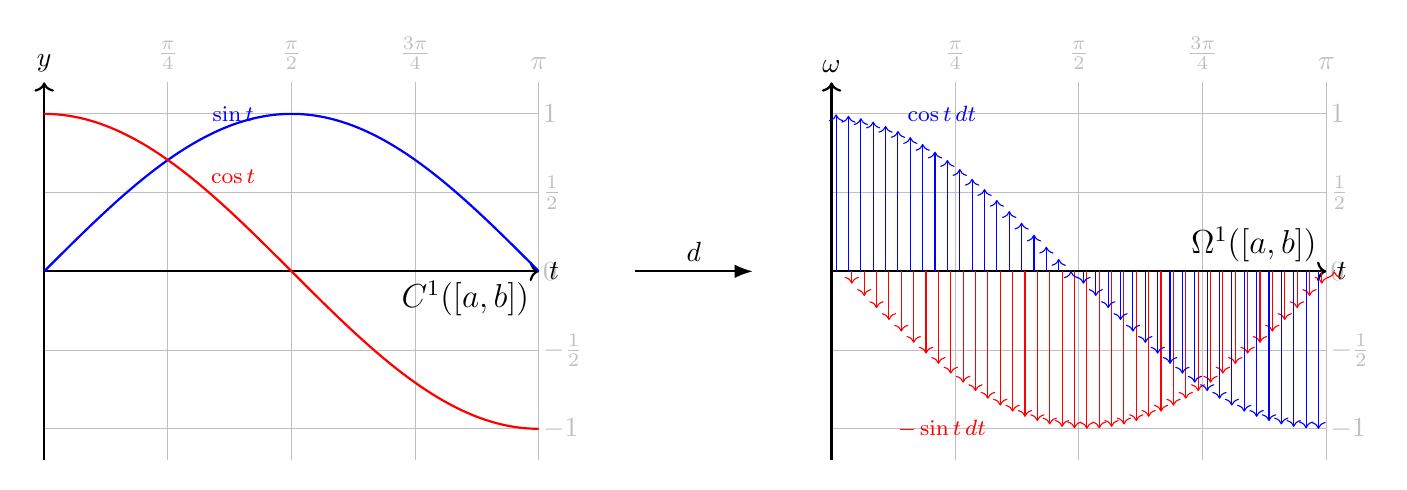
\begin{tikzpicture}[scale=2]
		% numeric constants
		\def\a{0}
		\def\b{3.141592653589793}             % π
		\def\topYmin{0}    \def\topYmax{1.2}
		\def\botYmin{-1.2}\def\botYmax{0}
		
		%── Top panel: C^1([a,b]) ──
		\begin{scope}[]
			% vertical grid lines at t = 0, π/4, π/2, 3π/4, π
			\foreach \x/\xlabel in {
				0.785/{$\tfrac{\pi}{4}$},
				1.570/{$\tfrac{\pi}{2}$},
				2.356/{$\tfrac{3\pi}{4}$},
				3.141/{$\pi$}
			}{
				\draw[lightgray,thin] (\x,-\topYmax) -- (\x,\topYmax)
				node[above,yshift=1pt] {\xlabel};
			}
			% horizontal grid lines at y = 0, 0.5, 1
			\foreach \y/\ylabel in {
				-1/{$-1$},
				-0.5/{$-\tfrac12$},
				0/{$0$},
				0.5/{$\tfrac12$},
				1/{$1$}
			}{
				\draw[lightgray,thin] (\a,\y) -- (\b,\y)
				node[right,xshift=-2pt] {\ylabel};
			}
			% axes
			\draw[->,thick] (\a,\topYmin) -- (\b,\topYmin) node[right] {$t$};
			\draw[->,thick] (\a,-\topYmax) -- (\a,\topYmax) node[above] {$y$};
			% the two C^1–curves
			\draw[blue,thick,domain=\a:\b,samples=200]
			plot (\x,{sin(\x r)});
			\draw[red,thick,domain=\a:\b,samples=200]
			plot (\x,{cos(\x r)});
			% labels
			\node at (\b,0) [below left] {\large $C^1([a,b])$};
			\node[blue] at (1.2,1.0) {\footnotesize$\sin t$};
			\node[red]  at (1.2,0.6) {\footnotesize$\cos t$};
		\end{scope}
		
		%── the exterior derivative arrow ──
		\draw[-Latex, thick] (3.75,0) to node[above] {$d$} (4.5,0);
		
		%── Bottom panel: Ω^1([a,b]) ──
		\begin{scope}[xshift=5cm]
			%── Bottom panel: Ω^1([a,b]) with 11 samples ──
			% grid lines (as before)
			\foreach \x/\xlabel in {
				0.785/{$\tfrac{\pi}{4}$},
				1.570/{$\tfrac{\pi}{2}$},
				2.356/{$\tfrac{3\pi}{4}$},
				3.141/{$\pi$}
			}{
				\draw[lightgray,thin] (\x,-\topYmax) -- (\x,\topYmax)
				node[above,yshift=1pt] {\xlabel};
			}
			% horizontal grid lines at y = 0, 0.5, 1
			\foreach \y/\ylabel in {
				-1/{$-1$},
				-0.5/{$-\tfrac12$},
				0/{$0$},
				0.5/{$\tfrac12$},
				1/{$1$}
			}{
				\draw[lightgray,thin] (\a,\y) -- (\b,\y)
				node[right,xshift=-2pt] {\ylabel};
			}
			% axes
			\draw[->,thick] (\a,0) -- (\b,0) node[right] {$t$};
			\draw[->,thick] (\a,-\topYmax) -- (\a,\topYmax) node[above] {$\omega$};
			
			% sample points t_k = k*pi/10, k=0..10
			\foreach \k in {0.25,0.5,...,10} {
				\pgfmathsetmacro{\x}{\k*pi/10}
				\pgfmathsetmacro{\yone}{cos(\x r)}
				\pgfmathsetmacro{\ytwo}{-sin(\x r)}
				% cos t dt on the left
				\draw[blue,->] ({\x-0.05},0) -- ++(0,{\yone});
				% -sin t dt on the right
				\draw[red,->]  ({\x+0.05},0) -- ++(0,{\ytwo});
			}
			
			% labels
			\node at (\b,\botYmax) [above left] {\large $\Omega^1([a,b])$};
			\node[blue] at (0.7,1) {\footnotesize$\cos t\,dt$};
			\node[red]  at (0.7,-1) {\footnotesize$-\sin t\,dt$};
		\end{scope}
	\end{tikzpicture}
\end{center}
The map \[
\fullfunction{d}{C^1([a,b])}{\Omega^1([a,b])}{f(t)}{d(f(t))=df}
\] is defined by $df=f'(t)dt$, where $f'$ is the derivative of $f$.


\begin{definition}[Space of Smooth Functions \(C^\infty(\R^n)\)]
	We write \(C^\infty(\R^n)\) for the set of all functions
	\[
	f:\R^n\;\longrightarrow\;\R
	\]
	that have continuous partial derivatives of every order.  Equivalently,
	\[
	C^\infty(\R^n)
	=\bigl\{\,f:\R^n\to\R\;\big|\;
	\text{for all multi‐indices }\alpha,\;
	\partial^\alpha f\text{ exists and is continuous}\bigr\},
	\]
	where \(\partial^\alpha f = \frac{\partial^{|\alpha|}f}{\partial x_1^{\alpha_1}\cdots\partial x_n^{\alpha_n}}\).
\end{definition}

\begin{definition}[Space of Smooth \(1\)–Forms on \(\R^n\)]
	We denote by \(C^\infty(\R^n)\) the set of all infinitely differentiable real‐valued functions on \(\R^n\).  A \emph{smooth \(1\)–form} is an expression of the form
	\[
	\omega
	= f_1(x)\,dx^1 \;+\; f_2(x)\,dx^2 \;+\;\cdots+\; f_n(x)\,dx^n,
	\]
	where each \(f_i\in C^\infty(\R^n)\) and \(dx^i\) are formal symbols.  The collection of all such forms is
	\[
	\Omega^1(\R^n)
	\;=\;
	\Bigl\{\,
	\sum_{i=1}^n f_i(x)\,dx^i
	\;\big|\;
	f_i(x)\in C^\infty(\R^n)
	\Bigr\}.
	\]
\end{definition}

\noindent\textbf{Remark.}  
- Each \(dx^i\) is thought of as “dual” to the partial derivative \(\partial/\partial x^i\).  
- Smooth \(1\)–forms can be integrated along curves (line integrals), since \(dx^i\) picks out the \(i\)th component of a tangent vector.  
- No notions of “open set” or “manifold” are needed at this level: we work directly in \(\R^n\).

%\begin{definition}[\(\Omega^1(U)\): Space of Smooth \(1\)–Forms]
%	Let \(U\subset\R^n\) be an open set.  The module of \emph{smooth \(1\)–forms} on \(U\) is
%	\[
%	\Omega^1(U)
%	\;=\;
%	\Bigl\{\,
%	\omega
%	=\sum_{i=1}^{n}f_i(x)\,dx^i
%	\;\Big|\;
%	f_i\in C^\infty(U)
%	\Bigr\},
%	\]
%	where each \(f_i\) is a smooth function on \(U\) and \(dx^i\) are the formal basis \(1\)–forms dual to the coordinate vector fields \(\partial/\partial x^i\).
%\end{definition}

%\begin{definition}[\(C^\infty\)–Functions]
%	Let \(U\subset\R^n\) be an open set.  The space
%	\[
%	C^\infty(U)
%	\;=\;
%	\bigl\{\,f:U\to\R : f\text{ is infinitely differentiable}\bigr\}
%	\]
%	is the \emph{algebra of smooth functions} on \(U\).  Equivalently, each \(f\in C^\infty(U)\) has continuous partial derivatives of all orders.  
%\end{definition}
%
%\begin{definition}[\(k\)\nobreakdash–Forms \(\Omega^k(U)\)]
%	On the same \(U\), the \(R\)\nobreakdash–module of smooth \emph{\(k\)–forms} is
%	\[
%	\Omega^k(U)
%	\;=\;
%	\Bigl\{\,
%	\omega
%	=\sum_{1\le i_1<\cdots<i_k\le n}
%	f_{i_1\cdots i_k}(x)\,
%	dx^{i_1}\wedge\cdots\wedge dx^{i_k}
%	\;\Big|\;
%	f_{i_1\cdots i_k}\in C^\infty(U)
%	\Bigr\}.
%	\]
%	Here \(dx^i\) are formal symbols and \(\wedge\) denotes the exterior (alternating) product.
%\end{definition}
\begin{remark}
	\ \begin{itemize}
		\item \(0\)–Forms are just smooth functions: \(\Omega^0(U)=C^\infty(U)\).
		\item A \(1\)–form \(\omega=f_1\,dx^1+\cdots+f_n\,dx^n\) can be naturally integrated along curves, yielding line integrals.
		\item A \(2\)–form in \(\R^3\), \(\alpha=P\,dy\wedge dz+Q\,dz\wedge dx+R\,dx\wedge dy\), encodes a flux density for surface integrals.
%		\item In general, a \(k\)–form is the appropriate integrand for integration over an oriented \(k\)–dimensional submanifold of \(U\).
%		\item The sequence
%		\[
%		0
%		\;\xrightarrow{\ } 
%		\Omega^0(U)
%		\;\xrightarrow{d}\;
%		\Omega^1(U)
%		\;\xrightarrow{d}\;
%		\cdots
%		\;\xrightarrow{d}\;
%		\Omega^n(U)
%		\;\xrightarrow{\ }0
%		\]
%		is the \emph{de\,Rham complex}, whose cohomology measures failure of exactness and underlies Stokes’ theorem.
	\end{itemize}
\end{remark}
\newpage
\section{Line and Surface Integrals as First Isomorphism Theorems}

We work on a smooth domain \(U\subset\R^2\) (for line integrals) or \(U\subset\R^3\) (for surface integrals), and use the exterior derivative
\[
d:\Omega^k(U)\;\longrightarrow\;\Omega^{k+1}(U).
\]

\begin{proposition}[Line Integrals and Exact 1-Forms]
	Let \(C\subset U\) be a piecewise \(C^1\) closed curve, and define the line‐integral functional
	\[
	I_C:\Omega^1(U)\;\longrightarrow\;\R,
	\qquad
	I_C(\alpha)=\oint_{C}\alpha.
	\]
	Then:
	\begin{enumerate}
		\item \(\displaystyle\ker I_C=\{\,\alpha\in\Omega^1(U):I_C(\alpha)=0\}\) coincides with \(\mathrm{im}(d)\), the space of exact \(1\)-forms, since by the Fundamental Theorem of Line Integrals
		\(\displaystyle I_C(df)=0\) for every \(f\in C^\infty(U)\).
		\item By the First Isomorphism Theorem for vector spaces,
		\[
		\Omega^1(U)\big/\!\mathrm{im}(d)
		\;\cong\;
		I_C\bigl(\Omega^1(U)\bigr)
		\;\subset\;\R.
		\]
	\end{enumerate}
	In particular, if \(C\) represents a generator of \(H_1(U;\Z)\cong\Z\), then \(I_C\bigl(\Omega^1(U)\bigr)=\R\) and
	\(\Omega^1(U)/\mathrm{im}(d)\cong\R\).
	
	\medskip
	
	\noindent\textbf{Example.}  On \(U=\R^2\setminus\{0\}\), let
	\[
	\alpha \;=\;
	-\frac{y}{x^2+y^2}\,dx \;+\;\frac{x}{x^2+y^2}\,dy.
	\]
	One checks \(d\alpha=0\) on \(U\), but \(\alpha\not\in\mathrm{im}(d)\).  The unit circle \(C\) generates \(H_1(U)\), and
	\[
	I_C(\alpha)
	=\oint_{C}\alpha
	=2\pi.
	\]
	Thus \(\alpha\) represents a nonzero class in 
	\(\Omega^1(U)/\mathrm{im}(d)\cong\R\).
	
\end{proposition}

\begin{proposition}[Surface Integrals and Exact 2-Forms]
	Let \(D\subset U\subset\R^3\) be a compact oriented surface with boundary \(\partial D\), and define the surface‐integral functional
	\[
	J_D:\Omega^2(U)\;\longrightarrow\;\R,
	\qquad
	J_D(\beta)=\iint_{D}\beta.
	\]
	Then:
	\begin{enumerate}
		\item \(\ker J_D=\mathrm{im}(d)\subset\Omega^2(U)\), since Stokes’ Theorem gives
		\(\displaystyle J_D(d\gamma)=\iint_D d\gamma = \oint_{\partial D}\gamma\), which vanishes whenever \(\gamma\) has compact support or \(\partial D\) is empty.
		\item By the First Isomorphism Theorem,
		\[
		\Omega^2(U)\big/\!\mathrm{im}(d)
		\;\cong\;
		J_D\bigl(\Omega^2(U)\bigr)
		\;\subset\;\R.
		\]
	\end{enumerate}
	
	\medskip
	
	\noindent\textbf{Example (Divergence Theorem).}
	In \(\R^3\), let \(\mathbf F=(P,Q,R)\) and identify the \(2\)-form
	\(\beta = P\,dy\wedge dz + Q\,dz\wedge dx + R\,dx\wedge dy\).  Then
	\[
	d\beta = \bigl(\partial_x P + \partial_y Q + \partial_z R\bigr)\,dx\wedge dy\wedge dz
	\]
	is the divergence form.  For a compact region \(D\) with boundary \(S=\partial D\),
	\[
	J_D(d\beta)
	=\iiint_D \mathrm{div}\,\mathbf F\,dV
	=\iint_S \mathbf F\cdot d\mathbf S,
	\]
	demonstrating that exactness of forms corresponds exactly to vanishing of flux by Gauss’s theorem.
	
\end{proposition}

\vfill
\section*{Level 1: The Fundamental Theorem of Calculus}

The equation
\[
\int_a^b \cos t \,\mathrm{d}t = \sin b - \sin a
\]
is a special case of the \textbf{Fundamental Theorem of Calculus}, which links differentiation and integration.

\begin{itemize}
	\item \(\displaystyle \int_a^b\): the \emph{definite integral}, representing the signed area under the integrand from \(t=a\) to \(t=b\).
	\item \(\cos t\): the \emph{integrand}, here the cosine function.
	\item \(t\): the \emph{variable of integration}.
	\item \(\mathrm{d}t\): the \emph{differential}, indicating integration with respect to \(t\).
	\item \(\sin b - \sin a\): the evaluation of the \emph{antiderivative} \(\sin t\) at the endpoints \(b\) and \(a\).
\end{itemize}

\medskip

\section*{Level 2: Line Integral of a Vector Field}

The line integral
\[
\int_{C} \bigl\langle -\tfrac{y}{r^2},\,\tfrac{x}{r^2}\bigr\rangle \cdot \mathrm{d}\mathbf{r}
\]
computes the {\em circulation} of the vector field \(\mathbf{F}(x,y)=\langle -y/r^2,\;x/r^2\rangle\) around the curve \(C\), taken here to be the unit circle \(x^2+y^2=1\).

\begin{itemize}
	\item \(\displaystyle \int_C\): integral \emph{along} a curve \(C\).
	\item \(C: x^2+y^2=1\): the \emph{unit circle}.
	\item \(\mathbf{F}(x,y)=\bigl\langle -y/r^2,\;x/r^2\bigr\rangle,\;r^2=x^2+y^2\).
	\item \(\mathrm{d}\mathbf{r}=\langle \mathrm{d}x,\mathrm{d}y\rangle\): the infinitesimal tangent vector.
	\item “\(\cdot\)”: the \emph{dot product}, measuring alignment of \(\mathbf{F}\) with \(\mathrm{d}\mathbf{r}\).
\end{itemize}

For this field, the result is
\(\displaystyle 2\pi\), 
indicating one full rotation around the origin.

\medskip

\section*{Level 3: Surface Integral of a Vector Field}

The surface integral
\[
\iint_{S}\mathbf F\cdot \mathrm{d}\mathbf S
\;=\;
\iint_{D}
\mathbf F\!\bigl(T(u,v)\bigr)
\;\cdot\;
\Bigl(\tfrac{\partial T}{\partial u}\times\tfrac{\partial T}{\partial v}\Bigr)
\,\mathrm{d}u\,\mathrm{d}v
\]
measures the \emph{flux} of \(\mathbf F\) through a parametrized surface \(S=T(D)\).

\begin{itemize}
	\item \(\displaystyle \iint_S\): surface integral over \(S\subset\R^3\).
	\item \(\mathrm{d}\mathbf S\): the vector area element, normal to \(S\).
	\item \(T(u,v)\): a smooth \emph{parametrization} of \(S\) by \((u,v)\in D\subset\R^2\).
	\item \(\tfrac{\partial T}{\partial u},\,\tfrac{\partial T}{\partial v}\): tangent vectors to \(S\).
	\item “\(\times\)”: cross product, giving the normal vector with magnitude equal to the area element.
	\item \(\mathrm{d}u\,\mathrm{d}v\): area element in parameter domain \(D\).
\end{itemize}

\medskip

\section*{Level 4: Abstract View with Differential Forms}

We summarize classical integrals in the language of differential forms and duality:

\medskip

\begin{tabular}{lll}
	\hline
	\textbf{Concept} & \textbf{Domain\(\to\)Target} & \textbf{Role} \\
	\hline
	Differential \(d\) & \(C^\infty(\R)\to\Omega^1(\R)\) 
	& \(f\mapsto f'(x)\,\mathrm{d}x\) \\
	Antiderivative \(I_{x_0}\) 
	& \(\Omega^1(\R)\to C^\infty(\R)\) 
	& \(\omega=f(x)\,\mathrm{d}x\mapsto\int_{x_0}^x f(t)\,\mathrm{d}t\) \\
	Integration \(\mathcal I_{[a,b]}\) 
	& \(\Omega^1(\R)\to\R\) 
	& \(\omega\mapsto\int_a^b\omega\) \\
	Dual module 
	& \(\Omega^1(\R)\to X(\R)\) 
	& 1-forms \(\leftrightarrow\) vector fields \\
	\hline
\end{tabular}

\begin{tabular}{lll}
	\hline
	\textbf{Concept} & \textbf{Domain\(\to\)Target} & \textbf{Role} \\
	\hline
	Differential \(d\) 
	& \(C^\infty(\R)\to\Omega^1(\R)\) 
	& \(f\mapsto f'(x)\,\mathrm{d}x\) \\[6pt]
	Antiderivative \(I_{x_0}\) 
	& \(\Omega^1(\R)\to C^\infty(\R)\) 
	& \(\omega=f(x)\,\mathrm{d}x\mapsto\displaystyle\int_{x_0}^x f(t)\,\mathrm{d}t\) \\[6pt]
	Integration \(\mathcal I_{[a,b]}\) 
	& \(\Omega^1(\R)\to\R\) 
	& \(\omega\mapsto\displaystyle\int_a^b\omega\) \\[6pt]
	Line integral \(I_C\) 
	& \(\Omega^1(\R^2)\to\R\) 
	& \(\alpha=P\,dx+Q\,dy\mapsto\displaystyle\oint_C\alpha
	=\oint_C\!P\,dx+Q\,dy\) \\[6pt]
	Surface integral \(J_S\) 
	& \(\Omega^2(\R^3)\to\R\) 
	& \(\beta=P\,dy\wedge dz+Q\,dz\wedge dx+R\,dx\wedge dy\mapsto\displaystyle\iint_S\beta
	=\iint_S\mathbf F\cdot d\mathbf S\) \\[6pt]
	Dual module 
	& \(\Omega^1(\R)\to X(\R)\) 
	& 1-forms \(\leftrightarrow\) vector fields \\
	\hline
\end{tabular}
\bigskip

\noindent
\textbf{\(C^\infty(\R)\)}: smooth functions.  
\quad 
\(\Omega^1(\R)\): space of 1-forms.  
\quad 
\(X(\R)\): space of vector fields.
\begin{remark}[FTC as a First Isomorphism Theorem for Differential Forms]
	Consider the exterior derivative
	\[
	d: C^\infty(\R)\;\longrightarrow\;\Omega^1(\R),
	\]
	which sends a smooth function \(f\) to the \(1\)\nobreakdash-form \(df=f'(x)\,dx\).  Then
	\[
	\ker(d)
	=\{\,f\in C^\infty(\R):df=0\}
	=\{\text{constant functions}\},
	\quad
	\mathrm{im}(d)
	=\{\,\omega\in\Omega^1(\R):\exists f,\ \omega=df\},
	\]
	the \emph{exact} \(1\)\nobreakdash-forms.  The \emph{First Isomorphism Theorem} for the ring homomorphism \(d\) gives
	\[
	C^\infty(\R)\big/\ker(d)
	\;\cong\;
	\mathrm{im}(d).
	\]
	On the other hand, the \emph{Fundamental Theorem of Calculus} asserts that for any exact form \(df\),
	\[
	\int_a^b df \;=\; f(b)-f(a),
	\]
	and that this assignment depends only on the class of \(f\) modulo constants.  Thus the map
	\[
	C^\infty(\R)\big/\ker(d)\;\longrightarrow\;\R,
	\qquad
	[f]\;\longmapsto\;f(b)-f(a),
	\]
	is precisely an inverse to the inclusion \(\mathrm{im}(d)\hookrightarrow\Omega^1(\R)\) composed with integration.  Equivalently, the FTC is the realization of the first isomorphism theorem in the category of differential forms.
\end{remark}

\newpage

\section{Line and Surface Integrals as First Isomorphism Theorems}

We work on a smooth domain \(U\subset\R^2\) (for line integrals) or \(U\subset\R^3\) (for surface integrals), and use the exterior derivative
\[
d:\Omega^k(U)\;\longrightarrow\;\Omega^{k+1}(U).
\]

\begin{proposition}[Line Integrals and Exact 1-Forms]
	Let \(C\subset U\) be a piecewise \(C^1\) closed curve, and define the line‐integral functional
	\[
	I_C:\Omega^1(U)\;\longrightarrow\;\R,
	\qquad
	I_C(\alpha)=\oint_{C}\alpha.
	\]
	Then:
	\begin{enumerate}
		\item \(\displaystyle\ker I_C=\{\,\alpha\in\Omega^1(U):I_C(\alpha)=0\}\) coincides with \(\mathrm{im}(d)\), the space of exact \(1\)-forms, since by the Fundamental Theorem of Line Integrals
		\(\displaystyle I_C(df)=0\) for every \(f\in C^\infty(U)\).
		\item By the First Isomorphism Theorem for vector spaces,
		\[
		\Omega^1(U)\big/\!\mathrm{im}(d)
		\;\cong\;
		I_C\bigl(\Omega^1(U)\bigr)
		\;\subset\;\R.
		\]
	\end{enumerate}
	In particular, if \(C\) represents a generator of \(H_1(U;\Z)\cong\Z\), then \(I_C\bigl(\Omega^1(U)\bigr)=\R\) and
	\(\Omega^1(U)/\mathrm{im}(d)\cong\R\).
	
	\medskip
	
	\noindent\textbf{Example.}  On \(U=\R^2\setminus\{0\}\), let
	\[
	\alpha \;=\;
	-\frac{y}{x^2+y^2}\,dx \;+\;\frac{x}{x^2+y^2}\,dy.
	\]
	One checks \(d\alpha=0\) on \(U\), but \(\alpha\not\in\mathrm{im}(d)\).  The unit circle \(C\) generates \(H_1(U)\), and
	\[
	I_C(\alpha)
	=\oint_{C}\alpha
	=2\pi.
	\]
	Thus \(\alpha\) represents a nonzero class in 
	\(\Omega^1(U)/\mathrm{im}(d)\cong\R\).
	
\end{proposition}

\begin{proposition}[Surface Integrals and Exact 2-Forms]
	Let \(D\subset U\subset\R^3\) be a compact oriented surface with boundary \(\partial D\), and define the surface‐integral functional
	\[
	J_D:\Omega^2(U)\;\longrightarrow\;\R,
	\qquad
	J_D(\beta)=\iint_{D}\beta.
	\]
	Then:
	\begin{enumerate}
		\item \(\ker J_D=\mathrm{im}(d)\subset\Omega^2(U)\), since Stokes’ Theorem gives
		\(\displaystyle J_D(d\gamma)=\iint_D d\gamma = \oint_{\partial D}\gamma\), which vanishes whenever \(\gamma\) has compact support or \(\partial D\) is empty.
		\item By the First Isomorphism Theorem,
		\[
		\Omega^2(U)\big/\!\mathrm{im}(d)
		\;\cong\;
		J_D\bigl(\Omega^2(U)\bigr)
		\;\subset\;\R.
		\]
	\end{enumerate}
	
	\medskip
	
	\noindent\textbf{Example (Divergence Theorem).}
	In \(\R^3\), let \(\mathbf F=(P,Q,R)\) and identify the \(2\)-form
	\(\beta = P\,dy\wedge dz + Q\,dz\wedge dx + R\,dx\wedge dy\).  Then
	\[
	d\beta = \bigl(\partial_x P + \partial_y Q + \partial_z R\bigr)\,dx\wedge dy\wedge dz
	\]
	is the divergence form.  For a compact region \(D\) with boundary \(S=\partial D\),
	\[
	J_D(d\beta)
	=\iiint_D \mathrm{div}\,\mathbf F\,dV
	=\iint_S \mathbf F\cdot d\mathbf S,
	\]
	demonstrating that exactness of forms corresponds exactly to vanishing of flux by Gauss’s theorem.
	
\end{proposition}

\end{document}
